\section{Methodology}
\label{sec:methodology}

In this section, we discuss the three algorithms used for distilling documents.
Two of our algorithms start by segmenting the document into smaller, contiguous, and exhaustive parts.
We do so by using a sentence tokenizer to separate sentences from the text and then merging them such that the number of words in each segment is more than the threshold $min\_words$, hyperparameter in both methods.


\subsection{Central Truncation}
\label{method:truncation}

Truncation is the most common and straightforward approach used to handle long texts that exceed the context size of an LLM.
It can be done in three main ways:

\begin{itemize}
  \item \textbf{Retaining Head}: Keeping tokens from the start.
  \item \textbf{Retaining Tail}: Keeping tokens from the end.
  \item \textbf{Head and Tail}: Keeping tokens from both start and end.
\end{itemize}

\citet{worsham-kalita-2018-genre} also employ "retaining head" and "retaining tail" strategies on long texts and find promising results for long text genre classification.
Though the "retaining head" method is often used, keeping the initial tokens allowed by the LLM, \citet{sun2019fine} find that keeping both head and tail produces better results than both the "retaining head" and the "retaining tail" methods.
Their research also shows that truncating the middle is even better than the more complicated hierarchical methods, displaying superiority with simplicity.
This is a time-efficient method worth exploring.

The fraction of tokens to be taken from the head is controlled by the hyperparameter $head\_size \in [0, 1]$ in our algorithm.
Setting $head\_size = 1$ results in taking tokens only from the head, whereas setting $head\_size = 0$ results in taking tokens only from the tail.
The truncated tokens are then sent to the model for summarization.


\subsection{Document Skimming}
\label{method:skimming}

\begin{figure*}[!ht]
  \centering
  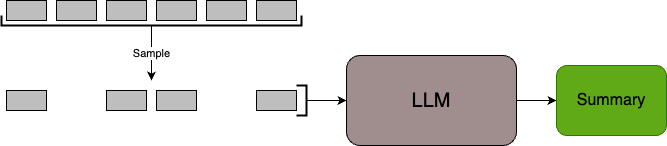
\includegraphics[width=.8\textwidth]{images/doc-skim.png}
  \caption{The Document Skimming Algorithm. The grey blocks represent segments of the document.}
  \label{fig:doc-skim}
\end{figure*}

One way to process long texts is by employing a speed reading strategy called skimming \cite{dhillon2020effect}.
Skimming is performed by reading the whole text in a go while selectively skipping some parts of the text for quicker reading.
The reader usually omits the portions that seem redundant or irrelevant in the text, minimizing information loss.
This method is inspired by the way \citet{wang2024videoagent} randomly sample video frames to generate captions.
\citet{worsham-kalita-2018-genre} also use random sampling for genre identification.

This method starts by segmenting the document with the hyperparameter $min\_words$ (introduced at the start of \autoref{sec:methodology}).
We then sample segments uniformly, with each segment having probability $p$ to be picked.
The sampled segments are then concatenated to form a single text and sent to the model.
This method ensures the model sees a segment from each part of the text.
\autoref{fig:doc-skim} is a visual representation of the algorithm.

Below is an example of the distilled text generated by the algorithm and the summary generated by GPT-3.5 Turbo \cite{brown2020language}:

\noindent \textbf{Example Text:}
\begin{quote}
  Title: Awards of Attorneys’ Fees by Federal Courts and Federal Agencies.
  Subsection I. Introduction: The American ...
\end{quote}

\noindent \textbf{Distilled Text:}
\begin{quote}
  Alyeska Pipeline Service Co. v. Wilderness Society , 421 U.S. 240, 247 (1975). This is known as the "American rule" (as opposed to the ...
\end{quote}

\noindent \textbf{Summary:}
\begin{quote}
  The American rule regarding attorneys' fees has two common law exceptions: the common benefit doctrine and bad faith ...
\end{quote}

Refer to \autoref{fig:uniform} to visualize the segments picked by the algorithm.

\begin{figure}
  \centering
  \includegraphics*[width=.45\textwidth]{images/uniform.png}
  \caption{Segments picked by the Document Skimming algorithm. Y-axis value of the ith segment
  on x-axis is 1 if its picked, 0 otherwise.}
  \label{fig:uniform}
\end{figure}

\subsubsection*{Removing Redundancy}

To address the issue of redundancy in the document, we experiment with and without removing redundant segments before and after sampling.
We do this to prevent the model from seeing the same information multiple times, which may lead to repetition in the output.
This is achieved by linearly iterating over the sampled segments and selectively removing some of the segments.
We do this by maintaining the mean embedding of the selected segments, initialized as a zero vector.
The current segment is retained if the cosine similarity between the mean embedding and the segment embedding is lower than a $threshold$, which acts as a hyperparameter.
A \href{https://huggingface.co/sentence-transformers/all-MiniLM-L6-v2}{sentence} transformer is used to generate the segment embeddings.
The sentence transformer is based on MiniLM \cite{wang2020minilm}, which is a distilled version of a larger encoder-only transformer model.
In case the current segment is retained, the mean embedding is updated as follows:

\[ new\_mean\_emb = \frac{n \cdot mean\_emb + seg\_emb}{n + 1} \]

\noindent where $n$ is the number of sampled segments (excluding the current segment),
$seg\_emb$ is the segment embedding of the current segment, $mean\_emb$ is the mean embedding, and $new\_mean$ is the updated mean embedding.

While removing segments after sampling, we waste some of the context size.
To alleviate this, we increase the probability of choosing a segment during sampling to compensate for the removed segments.
This fraction is controlled by the hyperparameter $prob\_boost$.
The updated probability is calculated as follows:

\[ p_{new} = (1 + prob\_boost) \cdot p \]

Even though removing redundant segments before sampling is less efficient due to the whole document being processed, it ensures better utilization of the LLM's context size.

\subsubsection*{Other Calculations}

We now discuss caluclation of the optimal value of $p$.
Let $X$ denote the total number of tokens in the sampled segments.
Since segments are sampled randomly, $X$ is a random variable.
If the context size of the model is $model\_size$, we want $\mathrm{E}[X] = model\_size$, where $\mathrm{E}[X]$ denotes the expectation of $X$.

Suppose we have $n \in \mathbb{N}$ segments and $X_i \sim \mathrm{Bernoulli}(p)$ denotes if segment $i$ is chosen, $i \in \{1, 2, \dots, n\}$.
If $len_i$ denotes the number of tokens in segment $i$, we can write:

\begin{align*}
  X &= \sum_{i = 1}^{n} X_i \cdot len_i \\
  \Rightarrow \mathrm{E}[X] &= \mathrm{E}[\sum_{i = 1}^{n} X_i \cdot len_i] \\
  &= \sum_{i = 1}^{n} \mathrm{E}[X_i \cdot len_i] \\
  &= \sum_{i = 1}^{n} \mathrm{E}[X_i] \cdot len_i
\end{align*}

Since $X_i \sim \mathrm{Bernoulli}(p)$ $\forall i \in \{1, 2, \dots, n\}$, we have $\mathrm{E}[X_i] = p$ $\forall i \in \{1, 2, \dots, n\}$.

\begin{align*}
  \therefore \mathrm{E}[X] &= \sum_{i = 1}^{n} p \cdot len_i \\
  &= p \cdot \sum_{i = 1}^{n} len_i
\end{align*}

Let $total\_len$ be the total number of tokens in the text, then $total\_len = \sum_{i = 1}^{n} len_i$.

\[ \therefore \mathrm{E}[X] = p \cdot total\_len = model\_size \]
\[ \Rightarrow p \cdot total\_len = model\_size \]
\[ \Rightarrow p = model\_size / total\_len \]


\subsection{Summarization with Keyword Extraction}
\label{method:keyword}

\begin{algorithm*}
  \caption{Summarization with Keyword Extraction}

  \begin{algorithmic}
    \State \textbf{Input:} $text$ (text), $size$ (context size of model)
    \State \textbf{Output:} Distilled text
    \State $segments \leftarrow \text{segmenter}(text)$
    \State $embeddings \leftarrow \text{sentence\_transformer}(segments)$
    \State $keywords \leftarrow \text{LDA}(text)$
    \State $\text{concatenate}(keywords, \text{delimiter})$
    \State $keyword\_embedding \leftarrow \text{sentence\_transformer}(keywords)$
    \State Sort $embeddings$ by decreasing cosine similarity scores with $keyword\_embedding$
    \State $selected \leftarrow \{\}$
    \State $num\_tokens \leftarrow 0$
    \For{$embedding \in embeddings$}
      \State $tokens \leftarrow \text{count\_tokens}(embedding)$
      \If{$tokens + num\_tokens \le size$}
        \State $selected \leftarrow selected \cup \{embedding\}$
        \State $num\_tokens += tokens$
      \EndIf
    \EndFor
    \State $\text{concatenate}(selected, \text{delimiter})$
    \State \Return{$selected$}
  \end{algorithmic}

  \label{algo:keyword}
\end{algorithm*}

Document skimming (\autoref{method:skimming}) involves a very intuitive and simple approach of sampling segments randomly.
In an attempt to use the entirety of the text, we experiment with an efficient keyword extraction algorithm to get important keywords that explain the core meaning of the document.
These keywords capture the overall meaning of the document and can help us sample segments intelligently, ensuring we get the most important segments from the document.

We use Latent Dirichlet Allocation (LDA) \cite{blei2003latent} with a single topic to get the topic words (or keywords) from the document.
There are many ways to use these to create a probability distribution to sample the segments.
A simple approach we use is to concatenate the keywords using a delimiter (a space is used in our experiments) to form a single sentence.
This sentence is then embedded to form the keyword embedding, which, in theory, captures a high-level meaning of the document.
The keyword sentence and document segments are embedded using the same \href{https://huggingface.co/sentence-transformers/all-MiniLM-L6-v2}{sentence transformer} used in the previous method.
The segment embeddings are then compared to the keyword embedding using cosine similarity to get similarity scores for each segment embedding.
The maximum possible number of segments with the highest similarity scores are retained.
The selected segments are then concatenated and sent to the model.
\autoref{algo:keyword} describes the process.

Below is an example of the distilled text generated by the algorithm and the summary generated by GPT-3.5 Turbo \cite{brown2020language}:

\noindent \textbf{Example Text:}
\begin{quote}
  Title: Awards of Attorneys’ Fees by Federal Courts and Federal Agencies. Subsection I. Introduction: The American ...
\end{quote}

\noindent \textbf{Distilled Text:}
\begin{quote}
  Title: Awards of Attorneys’ Fees by Federal Courts and Federal Agencies Subsection I. Introduction: The American Rule and ...
\end{quote}

\noindent \textbf{Summary:}
\begin{quote}
  The document discusses the American Rule regarding attorneys' fees, where prevailing litigants are not typically entitled to ...
\end{quote}

Refer to \autoref{fig:keyword} to visualize the segments picked by the algorithm.

\begin{figure}
  \centering
  \includegraphics*[width=.45\textwidth]{images/keyword.png}
  \caption{
    Segments picked by the Summarization with Keyword Extraction algorithm.
    Y-axis value of the ith segment on x-axis is 1 if its picked, 0 otherwise.
  }
  \label{fig:keyword}
\end{figure}

This approach is similar to the way \citet{golia2024action} use action items to pick segments of text (a neighbourhood of 2 sentences around the action item) to obtain meeting minutes.
